\documentclass[11pt,letterpaper]{article}
\usepackage[margin=0.85in,headheight=14pt]{geometry}
\usepackage{amsmath,amssymb}
\usepackage{enumitem}
\usepackage{fancyhdr}
\usepackage{lmodern}
\usepackage[T1]{fontenc}
\usepackage[dvipsnames]{xcolor}
\usepackage[most]{tcolorbox}
\usepackage{pgfplots}
\usepgfplotslibrary{groupplots}
\usetikzlibrary{arrows.meta,positioning,shapes.geometric}
\pgfplotsset{
  compat=1.18,
  every axis/.append style={grid=major, grid style={gray!25}, tick label style={font=\footnotesize},
    label style={font=\small}, title style={font=\small}, legend style={font=\scriptsize}},
}
\definecolor{cA}{HTML}{1F77B4}
\definecolor{cB}{HTML}{FF7F0E}
\definecolor{cC}{HTML}{2CA02C}
\definecolor{cD}{HTML}{D62728}
\definecolor{cE}{HTML}{9467BD}

\pagestyle{fancy}
\fancyhf{}
\lhead{SYDE 556/750 \qquad Practice Test 3}
\rhead{Solutions \& marking guide}
\cfoot{\thepage}
\renewcommand{\headrulewidth}{0pt}

\setlength{\parindent}{0pt}
\setlength{\parskip}{4pt}

\newcommand{\tref}{\tau_{\mathrm{ref}}}
\newcommand{\trc}{\tau_{RC}}
\newcommand{\tin}{\tau_{\mathrm{in}}}
\newcommand{\T}{\mathsf T}
\newcommand{\ans}[1]{\par\vspace{4pt}{\bfseries #1}\quad}

\newtcolorbox{result}{colback=Green!6,colframe=Green!50!black,boxrule=0.5pt,left=4pt,right=4pt,top=2pt,bottom=2pt,arc=1pt}
\newtcolorbox{marking}{colback=blue!3,colframe=blue!40!black,boxrule=0.4pt,left=4pt,right=4pt,top=2pt,bottom=2pt,arc=1pt,fonttitle=\bfseries\small,title=Marking}
\newtcolorbox{trap}{colback=red!4,colframe=red!50!black,boxrule=0.4pt,left=4pt,right=4pt,top=2pt,bottom=2pt,arc=1pt,fonttitle=\bfseries\small,title=Where marks are usually lost}

\begin{document}

\begin{center}
{\Large\bfseries Practice Test 3: Solutions \& Marking Guide}\\[2pt]
Total: 20 marks plus 2 bonus. Open this guide only after attempting the paper under test conditions.\\
Follow-through credit applies to a clear method after a minor earlier error.
\end{center}

%=====================================================================
\section*{Question 1 \hfill (4)}

\ans{(a) [2]}
Use the Laplace transform. The two properties needed are that convolution becomes multiplication and that $d/dt$ becomes multiplication by $s$ (for signals starting at zero). The synapse transforms to
\[
H(s) = \int_0^\infty \tfrac1\tau e^{-t/\tau}e^{-st}dt = \frac{1}{1 + s\tau}.
\]
Then
\[
X = \frac{G + F}{1 + s\tau} \ \Rightarrow\ X + s\tau X = G + F \ \Rightarrow\ s\tau X = G + F - X \ \Rightarrow\ \boxed{\ \dot x = \tfrac1\tau\bigl(g(u) + f(x) - x\bigr)\ }
\]
\begin{marking}
0.5: names the Laplace transform and both properties. \ 0.5: $H(s) = 1/(1 + s\tau)$ (evaluated or correctly quoted). \ 1: algebra to the final ODE, including the $-x$ term. A correct time-domain derivation (differentiating the convolution integral) earns full marks.
\end{marking}

\ans{(b) [2]}
$\tau\dot x = u - x - x = 1 - 2x$, so $\dot x = \frac{1}{\tau/2}\bigl(\tfrac12 - x\bigr)$ and
\[
x(t) = \tfrac12\bigl(1 - e^{-t/(10\,\mathrm{ms})}\bigr).
\]
The steady state is $\tfrac12$ and the time constant is $\tau/2 = 10$ ms, twice as fast as the synapse alone.
\begin{center}
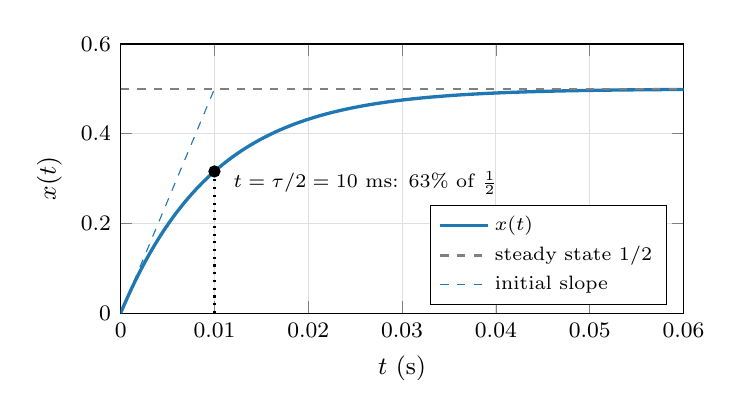
\begin{tikzpicture}
\begin{axis}[width=0.72\textwidth, height=5cm, xmin=0, xmax=0.06, ymin=0, ymax=0.6,
  xlabel={$t$ (s)}, ylabel={$x(t)$}, scaled x ticks=false, xticklabel style={/pgf/number format/fixed},
  legend pos=south east, legend cell align=left]
  \addplot[cA, very thick, domain=0:0.06, samples=150] {0.5*(1-exp(-x/0.01))};
  \addplot[gray, dashed, thick, domain=0:0.06, samples=2] {0.5};
  \addplot[cA, thin, dashed, domain=0:0.01, samples=2] {50*x};
  \legend{$x(t)$, steady state $1/2$, initial slope}
  \addplot[only marks, mark=*, black, forget plot] coordinates {(0.01,0.316)};
  \draw[dotted, thick] (axis cs:0.01,0) -- (axis cs:0.01,0.316);
  \node[font=\scriptsize, anchor=west] at (axis cs:0.011,0.29) {$t = \tau/2 = 10$ ms: $63\%$ of $\tfrac12$};
\end{axis}
\end{tikzpicture}
\end{center}
\begin{marking}
0.5: starts at $0$ and rises concavely (steepest at $t = 0$), no overshoot. \ 0.5: asymptote $\tfrac12$ labelled. \ 0.5: time constant $10$ ms labelled (as $\tau/2$ or $63\%$ point). \ 0.5: axes labelled with units. A steady state of $1$ or time constant $20$ ms loses the corresponding half-mark.
\end{marking}
\begin{trap}
The steady-state guess $x = u - x$ gives $\tfrac12$ but not the speed. The time constant is not the synapse's $20$ ms: the feedback $-x$ doubles the leak.
\end{trap}

%=====================================================================
\section*{Question 2 \hfill (4)}

\ans{(a) [2]}
$A = 0$, $B = 1$. With $A' = \tau A + I$ and $B' = \tau B$: $A' = 1$ and $B' = \tau = 0.1$.
\begin{center}
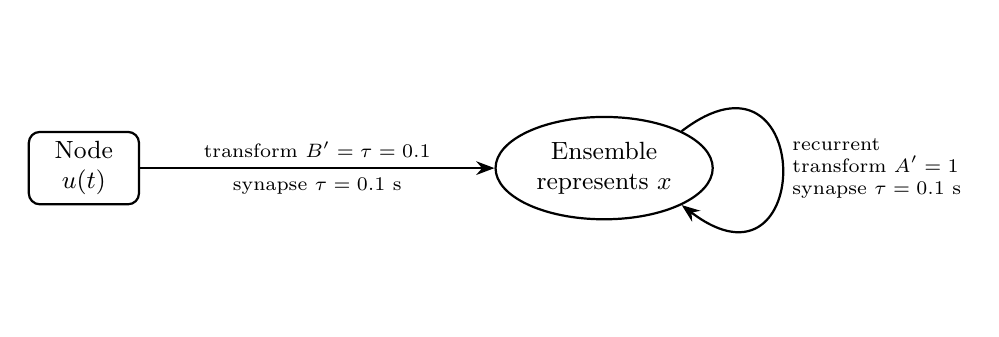
\begin{tikzpicture}[font=\small,
  box/.style={draw, thick, rounded corners, minimum height=0.9cm, minimum width=1.4cm, align=center}]
  \node[box] (u) {Node\\$u(t)$};
  \node[box, ellipse, right=4.5cm of u, minimum width=2.4cm, minimum height=1.3cm] (x) {Ensemble\\represents $x$};
  \draw[-{Stealth}, thick] (u) -- node[above, font=\scriptsize] {transform $B' = \tau = 0.1$} node[below, font=\scriptsize] {synapse $\tau = 0.1$ s} (x);
  \draw[-{Stealth}, thick] (x.north east) .. controls +(1.7,1.3) and +(1.7,-1.3) .. (x.south east)
    node[pos=0.5, right, font=\scriptsize, align=left] {recurrent\\transform $A' = 1$\\synapse $\tau = 0.1$ s};
\end{tikzpicture}
\end{center}
\begin{marking}
0.5: $A = 0$, $B = 1$. \ 0.5: $A' = 1$, $B' = 0.1$. \ 1: diagram with an input connection and a recurrent connection back onto the same ensemble, each labelled with transform and synapse. Swapping $A'$ and $B'$ loses the second half-mark.
\end{marking}

\ans{(b) [2]}
\[
x(t) = \int_0^t u(t')\,dt' = \begin{cases}
0, & t < 0.1,\\
0.5(t - 0.1), & 0.1 \le t < 0.5,\\
0.2 - (t - 0.5), & 0.5 \le t < 0.7,\\
0, & t \ge 0.7.
\end{cases}
\]
Check the joins: at $t = 0.5$, $0.5(0.4) = 0.2$; at $t = 0.7$, $0.2 - 0.2 = 0$.
\begin{center}
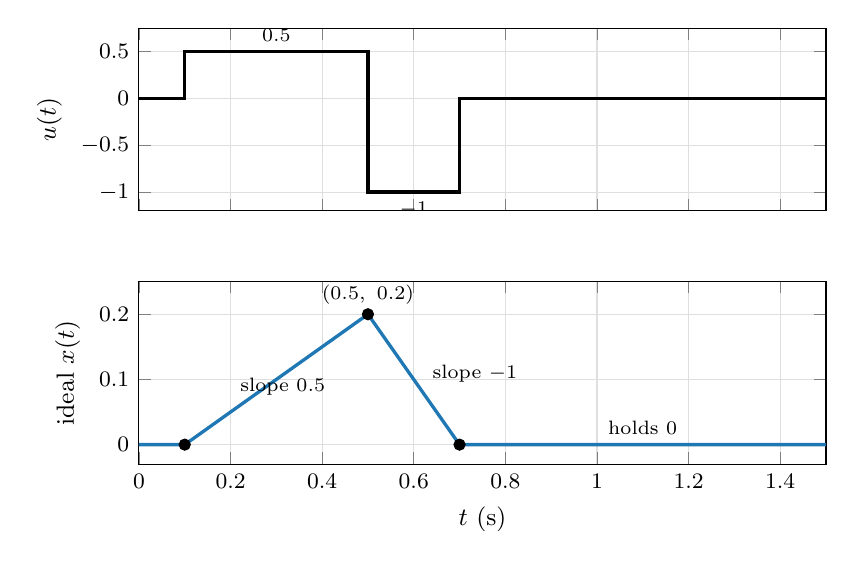
\begin{tikzpicture}
\begin{groupplot}[group style={group size=1 by 2, vertical sep=0.9cm, xticklabels at=edge bottom},
  width=0.85\textwidth, height=3.9cm, xmin=0, xmax=1.5]
\nextgroupplot[ylabel={$u(t)$}, ymin=-1.2, ymax=0.75]
  \addplot[black, very thick] coordinates {(0,0) (0.1,0) (0.1,0.5) (0.5,0.5) (0.5,-1) (0.7,-1) (0.7,0) (1.5,0)};
  \node[font=\scriptsize, anchor=south] at (axis cs:0.3,0.5) {$0.5$};
  \node[font=\scriptsize, anchor=north] at (axis cs:0.6,-1) {$-1$};
\nextgroupplot[ylabel={ideal $x(t)$}, xlabel={$t$ (s)}, ymin=-0.03, ymax=0.25]
  \addplot[cA, very thick] coordinates {(0,0) (0.1,0) (0.5,0.2) (0.7,0) (1.5,0)};
  \addplot[only marks, mark=*, black] coordinates {(0.1,0) (0.5,0.2) (0.7,0)};
  \node[font=\scriptsize, anchor=south] at (axis cs:0.5,0.2) {$(0.5,\ 0.2)$};
  \node[font=\scriptsize, anchor=south west] at (axis cs:0.2,0.06) {slope $0.5$};
  \node[font=\scriptsize, anchor=south west] at (axis cs:0.62,0.08) {slope $-1$};
  \node[font=\scriptsize, anchor=south] at (axis cs:1.1,0) {holds $0$};
\end{groupplot}
\end{tikzpicture}
\end{center}
\begin{marking}
1: all four cases, each starting from the previous end value, with no integration constant (0.5 for the middle two cases, 0.5 for the outer two). \ 1: aligned sketch with correct slopes, peak $0.2$ at $t = 0.5$, return to $0$ at $t = 0.7$, flat afterward, axes labelled.
\end{marking}
\begin{trap}
Writing $x = -t$ on the third piece (forgetting it starts from $0.2$), and drawing $x$ dropping back to zero when $u$ turns off. An integrator holds its value when $u = 0$.
\end{trap}

%=====================================================================
\section*{Question 3 \hfill (4)}

\ans{(a) [2]}
$\tau\dot x = u + f(x) - x = 2x - x^3 - x = x - x^3 = x(1 - x)(1 + x)$. Equilibria: $x = 0, \pm 1$.
With $\tau\phi'(x) = 1 - 3x^2$: at $x = 0$ it is $+1$, so $0$ is unstable. At $x = \pm1$ it is $-2$, so $\pm1$ are stable.
\begin{marking}
0.5: correct $\dot x = (x - x^3)/\tau$, including the $-x$ leak. \ 0.5: all three equilibria. \ 1: correct stability with a reason (sign of $\phi'$, or arrows on each side). Classifying with the algebraic $x = f(x)$ alone earns no stability marks.
\end{marking}

\ans{(b) [2]}
Between $0$ and $1$, $\dot x > 0$ (moves right); beyond $1$, $\dot x < 0$ (moves left). The picture is mirrored for negative $x$. With $u = 0$ the state is pushed away from $0$ to whichever of $\pm1$ is on its side:
\[
x(t) = \frac{x_0e^{t/\tau}}{\sqrt{1 - x_0^2 + x_0^2e^{2t/\tau}}}.
\]
\begin{center}
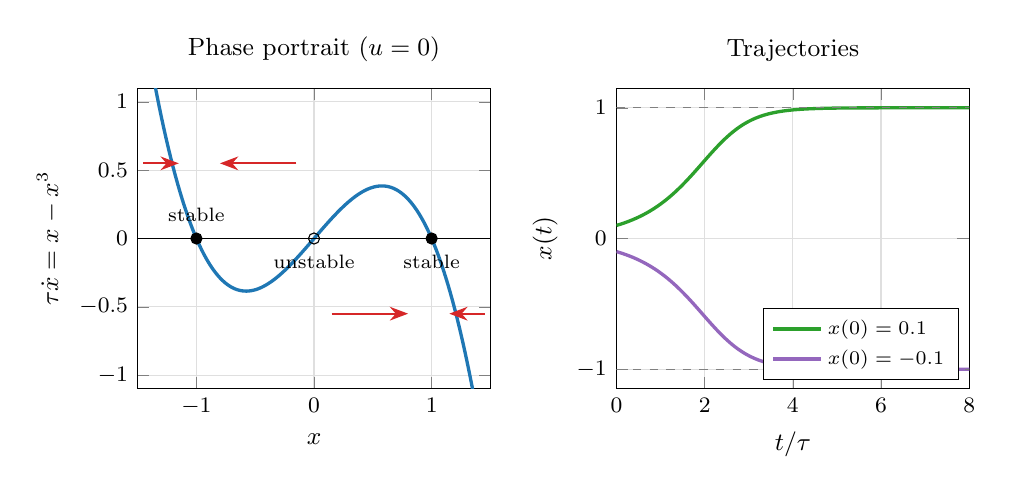
\begin{tikzpicture}
\begin{groupplot}[group style={group size=2 by 1, horizontal sep=1.6cm}, width=0.5\textwidth, height=5.4cm]
\nextgroupplot[xmin=-1.5, xmax=1.5, ymin=-1.1, ymax=1.1, xlabel={$x$}, ylabel={$\tau\dot x = x - x^3$}, title={Phase portrait ($u = 0$)}]
  \addplot[cA, very thick, domain=-1.5:1.5, samples=150] {x - x^3};
  \addplot[black, domain=-1.5:1.5, samples=2] {0};
  \addplot[only marks, mark=*, black] coordinates {(-1,0) (1,0)};
  \addplot[only marks, mark=o, black, mark options={fill=white}] coordinates {(0,0)};
  \draw[-{Stealth}, thick, cD] (axis cs:0.15,-0.55) -- (axis cs:0.8,-0.55);
  \draw[-{Stealth}, thick, cD] (axis cs:1.45,-0.55) -- (axis cs:1.15,-0.55);
  \draw[-{Stealth}, thick, cD] (axis cs:-0.15,0.55) -- (axis cs:-0.8,0.55);
  \draw[-{Stealth}, thick, cD] (axis cs:-1.45,0.55) -- (axis cs:-1.15,0.55);
  \node[font=\scriptsize, anchor=north] at (axis cs:1,-0.05) {stable};
  \node[font=\scriptsize, anchor=south] at (axis cs:-1,0.05) {stable};
  \node[font=\scriptsize, anchor=north] at (axis cs:0,-0.05) {unstable};
\nextgroupplot[xmin=0, xmax=8, ymin=-1.15, ymax=1.15, xlabel={$t/\tau$}, ylabel={$x(t)$}, title={Trajectories}, legend pos=south east, legend cell align=left]
  \addplot[cC, very thick, domain=0:8, samples=150] {0.1*exp(x)/sqrt(1-0.01+0.01*exp(2*x))};
  \addplot[cE, very thick, domain=0:8, samples=150] {-0.1*exp(x)/sqrt(1-0.01+0.01*exp(2*x))};
  \addplot[gray, dashed, domain=0:8, samples=2, forget plot] {1};
  \addplot[gray, dashed, domain=0:8, samples=2, forget plot] {-1};
  \legend{$x(0) = 0.1$, $x(0) = -0.1$}
\end{groupplot}
\end{tikzpicture}
\end{center}
It is a memory because with no input the state stays at $+1$ or $-1$ indefinitely, so the network stores which way it was last pushed (one bit).
\begin{marking}
1: cubic shape with three zeros and correctly directed arrows, stable and unstable points marked, axes labelled. \ 0.5: both trajectories leave $\pm0.1$ slowly at first, then turn over and settle at $\pm1$ (S-shaped, no crossing of zero). \ 0.5: memory sentence (persistence without input, history-dependent). Exact timing is not required.
\end{marking}

%=====================================================================
\section*{Question 4 \hfill (4)}

\ans{(a) [2]}
\begin{itemize}[leftmargin=1.2em]
\item \textbf{Static distortion (decoder error).} The recurrent decoder gives $\hat f'(x) \ne x$, so the real dynamics are $\dot x = (\hat f'(x) - x)/\tau \ne 0$. This has small stable and unstable zeros, and the state drifts deterministically toward the nearest stable one. That is the repeatable rate-mode drift.
\item \textbf{Spike noise.} Spikes make the filtered activity fluctuate, so the state takes a random walk. That is why spiking runs wander and end at different values.
\end{itemize}
More neurons reduce both. Static distortion shrinks roughly as $1/n$ (in RMSE), so the drift slows. Spike noise averages out roughly as $1/\sqrt n$, so the random walk shrinks. Neither reaches zero.
\begin{center}
\begin{tikzpicture}
\begin{axis}[width=0.9\textwidth, height=5.6cm, xmin=0, xmax=1.5, ymin=-0.12, ymax=0.3,
  xlabel={$t$ (s)}, ylabel={represented $x$}, legend pos=north east, legend cell align=left,
  title={Nengo, 200 neurons, $\tau = 0.1$ s, $\tin = 5$ ms, probe $10$ ms}]
  \addplot[black, very thick, dashed] table[x=t, y=ideal] {pn3_data/integrator_test.dat};
  \addplot[cA, thick] table[x=t, y=spike1] {pn3_data/integrator_test.dat};
  \addplot[cB, thick] table[x=t, y=spike2] {pn3_data/integrator_test.dat};
  \addplot[cC, very thick] table[x=t, y=rate] {pn3_data/integrator_test.dat};
  \legend{ideal $\int u$, spiking run 1, spiking run 2, rate mode}
\end{axis}
\end{tikzpicture}
\end{center}
After $t = 0.7$ s the spiking traces wander around differently, while the rate trace drifts smoothly and slowly. The offset during the input is part (b).
\begin{marking}
0.5 + 0.5: each source named. \ 0.5: correct mapping (distortion gives the deterministic drift that survives rate mode; spike noise gives the run-to-run variation). \ 0.5: both shrink with more neurons. Saying ``noise'' for both sources earns at most 1.
\end{marking}

\ans{(b) [2]}
With $A' = 1$ and $B' = \tau$:
\[
X = \frac{X}{1 + s\tau} + \frac{\tau U}{1 + s\tin}
\ \Rightarrow\ X\frac{s\tau}{1 + s\tau} = \frac{\tau U}{1 + s\tin}
\ \Rightarrow\ X = \frac{1 + s\tau}{1 + s\tin}\cdot\frac{U}{s}.
\]
Since $\frac{1 + s\tau}{1 + s\tin} = 1 + \frac{s(\tau - \tin)}{1 + s\tin}$,
\[
X = \frac{U}{s} + (\tau - \tin)\frac{U}{1 + s\tin}, \qquad x(t) = \int_0^t u + (\tau - \tin)\,(h_{\tin} * u)(t).
\]
The integral is exact. On top of it, the input leaks into the state, filtered by $5$ ms and weighted by $\tau - \tin = 0.095$ s:
\begin{itemize}[leftmargin=1.2em]
\item $0.1 \le t < 0.5$: about $+0.095 \times 0.5 \approx +0.048$ above the ideal (so about $0.25$ instead of $0.2$ at $t = 0.5$);
\item $0.5 \le t < 0.7$: about $-0.095$ below the ideal;
\item after $0.7$: the offset decays within a few ms (several $\tin$) and the final value is the ideal $0$.
\end{itemize}
Each jump of $u$ produces a quick step of $0.095\,\Delta u$ in the trace, smoothed over about $5$ ms.
\begin{center}
\begin{tikzpicture}
\begin{axis}[width=0.9\textwidth, height=5.6cm, xmin=0, xmax=1.0, ymin=-0.12, ymax=0.3,
  xlabel={$t$ (s)}, ylabel={$x$}, legend pos=north east, legend cell align=left,
  title={Prediction from (b) against the simulation}]
  \addplot[black, very thick, dashed] table[x=t, y=ideal] {pn3_data/integrator_test.dat};
  \addplot[cD, very thick] table[x=t, y=lead] {pn3_data/integrator_test.dat};
  \addplot[cC, thick] table[x=t, y=rate] {pn3_data/integrator_test.dat};
  \legend{ideal $\int u$, predicted $\int u + 0.095\,(h_{\tin} * u)$, Nengo rate mode}
  \draw[{Stealth}-{Stealth}] (axis cs:0.35,0.125) -- (axis cs:0.35,0.1725);
  \node[font=\scriptsize, anchor=east] at (axis cs:0.345,0.15) {$+0.048$};
  \draw[{Stealth}-{Stealth}] (axis cs:0.62,0.08) -- (axis cs:0.62,-0.015);
  \node[font=\scriptsize, anchor=west] at (axis cs:0.625,0.035) {$-0.095$};
\end{axis}
\end{tikzpicture}
\end{center}
The simulated trace follows the prediction, plus the smoothing of the $10$ ms probe filter.
\begin{marking}
1: correct Laplace setup with two different filters and algebra to the stated form. \ 0.5: offset $(\tau - \tin)u$ with sizes $\approx +0.048$ and $-0.095$. \ 0.5: offset disappears after the input ends; the final value is unaffected.
\end{marking}
\begin{trap}
Claiming the only effect is ``a small $5$ ms lag''. The leak-through term is $19$ times larger than $\tin$ would suggest, because it is weighted by $\tau - \tin$.
\end{trap}

%=====================================================================
\section*{Question 5 \hfill (4)}

\ans{(a) [1]}
$\mathrm{RMSE} = 3\varepsilon$. Nengo represents $x/r$ internally with the same neurons, so the normalized decoding problem is identical and the decoded output, including its error, is multiplied by $r$.
\begin{marking}
0.5: $3\varepsilon$ (or $\mathrm{RMSE} \propto r$). \ 0.5: the scaling reason.
\end{marking}

\ans{(b) [2]}
With intercept and maximum rate fixed, $J(x) = 1 + (J^{\max} - 1)\frac{0.5 - x}{1.5}$ for $x < 0.5$, where $J^{\max} = \bigl(1 - e^{(\tref - 1/200)/\trc}\bigr)^{-1}$: $\approx 5.5$ for $\tref = 1$ ms and $\approx 20.5$ for $4$ ms. Both curves are $0$ for $x \ge 0.5$ and reach $200$ Hz at $x = -1$. The $4$ ms curve shoots up just left of the intercept and then flattens, because at $200$ Hz it is close to its $1/\tref = 250$ Hz ceiling. The $1$ ms curve (ceiling $1000$ Hz) is much straighter.
\begin{center}
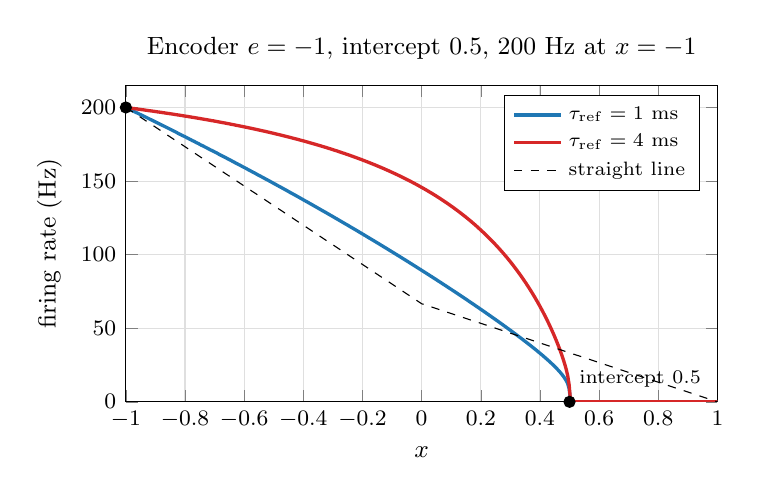
\begin{tikzpicture}[
  declare function={lif(\z,\tr,\tc,\Jm) = (\z > 0) * 1/(\tr - \tc*ln(1 - 1/(1 + (\Jm-1)*max(\z,1e-6))));}]
\begin{axis}[width=0.75\textwidth, height=5.6cm, xmin=-1, xmax=1, ymin=0, ymax=215,
  xlabel={$x$}, ylabel={firing rate (Hz)}, legend pos=north east, legend cell align=left,
  title={Encoder $e = -1$, intercept $0.5$, $200$ Hz at $x = -1$}]
  \addplot[cA, very thick, domain=-1:1, samples=400] {lif((0.5-x)/1.5,0.001,0.02,5.5167)};
  \addplot[cD, very thick, domain=-1:1, samples=400] {lif((0.5-x)/1.5,0.004,0.02,20.504)};
  \addplot[black, dashed, domain=-1:1, samples=3] {200*max((0.5-x)/1.5,0)};
  \legend{$\tref = 1$ ms, $\tref = 4$ ms, straight line}
  \addplot[only marks, mark=*, black, forget plot] coordinates {(0.5,0) (-1,200)};
  \node[font=\scriptsize, anchor=south west] at (axis cs:0.5,3) {intercept $0.5$};
\end{axis}
\end{tikzpicture}
\end{center}
The population with the larger $\tref$ has the larger RMSE. Its more curved, saturating tuning curves are worse building blocks for the straight line $\hat x = x$. Nengo, for 100 neurons: about $0.0053$ at $1$ ms against $0.0069$ at $4$ ms.
\begin{marking}
0.5: both curves decrease toward the right, zero for $x \ge 0.5$ (correct encoder direction). \ 0.5: same intercept and same $200$ Hz endpoint at $x = -1$; $4$ ms curve visibly more concave. \ 1: larger $\tref$ gives larger RMSE, with a reason linking curvature or saturation to decoding error. Drawing ReLU-style straight lines loses the shape half-mark.
\end{marking}

\ans{(c) [1]}
\[
v = (0.2, 0.5) - 2(0.3, -0.1) + 3(0.1, 0.2) = (0.2 - 0.6 + 0.3,\ 0.5 + 0.2 + 0.6) = (-0.1,\ 1.3),
\]
so $\|v\| = \sqrt{1.70} \approx 1.30$.
This lies outside the radius-$1$ disc, so $\hat v$ will be inaccurate: the second component falls short and the error is far larger than inside the trained range. Fix: give $v$ a radius of at least about $1.3$ (for example $1.5$), or scale the transforms down and rescale downstream.
\begin{marking}
0.5: $v = (-0.1, 1.3)$. \ 0.5: notes $\|v\| > 1$ and gives a valid fix. Checking only the components against $1$ is acceptable here, since $1.3 > 1$ either way.
\end{marking}

%=====================================================================
\section*{Bonus Question 1 \hfill (2)}
The synapse is a leaky integrator. It drifts toward whatever input it receives and forgets its own value with time constant $\tau$. The ``$+I$'' feeds the current state back into the population, which exactly replaces what the synapse leaks away, so with nothing else added the state holds. Multiplying by $\tau$ converts the desired rate of change into the input the slow synapse needs, because a synapse moves by (input $-$ state)$/\tau$ per second. A feed-forward chain has no such loop. Each population's state is just its filtered input, so it decays within a few synaptic time constants (tens of milliseconds) after the input stops.
\begin{marking}
0.5: synapse as leaky integrator / forgetting. \ 0.5: $+I$ cancels the leak. \ 0.5: $\tau$ scaling as converting a rate into the synapse's input. \ 0.5: feed-forward forgets within a few $\tau$.
\end{marking}

\end{document}
